\lstdefinestyle{mystyle}{
  backgroundcolor=\color{backcolour},   commentstyle=\color{codegreen},
  keywordstyle=\color{magenta},
  numberstyle=\tiny\color{codegray},
  stringstyle=\color{codepurple},
  basicstyle=\ttfamily\footnotesize,
  breakatwhitespace=false,         
  breaklines=true,                 
  captionpos=b,                    
  keepspaces=true,                 
  numbers=left,                    
  numbersep=5pt,                  
  showspaces=false,                
  showstringspaces=false,
  showtabs=false,                  
  tabsize=2
}

\section{Appendix}
\label{ch:appendix}

\subsection{Content of enclosed CD}
All codes are on the CD, frontend, backend, database, stored in the 'movie\_RS' folder directory. The electronic version of the thesis is stored in the 'thesis' folder directory.
\subsection{Kernel Code}

\lstset{style=mystyle}


\begin{lstlisting}[language=Python, caption=generate\_path]

def forward(self, x, path_index):
        if self.training:
            path_num = path_index.shape[1]
            path_index = path_index[:, np.random.choice(range(path_num), int(path_num * (1 - self.path_dropout)))]
        x = F.dropout(x, p=self.dropout, training=self.training)
        x = F.elu(self.conv1(x, path_index)[0])
        x = F.dropout(x, p=self.dropout, training=self.training)
        x, att = self.conv2(x, path_index)
        return x, att

\end{lstlisting}

\begin{lstlisting}[language=Python, caption=build\_user]

def build_user(self, iids, demographic_info):
        """
        Build user profiles given the historical user interactions
        :param iids: user selected item ids, list
        :param demographic_info: (gender, occupation), tuple
        :return:
        """
        self.base_iids = iids
        self.demographic_info = demographic_info
        # Build edges for new user
        self.new_user_nid = self.model.node_emb.weight.shape[0]

        new_user_gender_nid = self.data.e2nid[0]['gender'][demographic_info[0]]
        new_user_occ_nid = self.data.e2nid[0]['occ'][int(demographic_info[1])]
        i_nids = [self.data.e2nid[0]['iid'][iid] for iid in iids]
        row = i_nids + [new_user_gender_nid, new_user_occ_nid]
        col = [self.new_user_nid for i in range(len(iids) + 2)]
        self.new_edge_index = torch.from_numpy(np.array([row, col])).long().to(self.device_args['device'])

        # Build path begins and ends with
        new_path_np = utils.path.join(self.data.edge_index, self.new_edge_index)
        self.new_path = torch.from_numpy(new_path_np).long().to(self.device_args['device'])

        # Get new user embedding by applying message passing
        self.new_user_emb = torch.nn.Embedding(1, self.model.node_emb.weight.shape[1], max_norm=1, norm_type=2.0)
        new_node_emb = torch.cat((self.model.node_emb.weight, self.new_user_emb.weight), dim=0)
        self.propagated_new_user_emb = self.model(new_node_emb, self.new_path)[0][-1, :]

\end{lstlisting}

\begin{lstlisting}[language=Python, caption=get\_recommendation]

def get_recommendations(self,rs_proportion):

        iids = self.get_top_n_popular_items(500).iid
        iids = [iid for iid in iids if iid not in self.recommended]
        rec_iids = [iid for iid in iids if iid not in self.base_iids]
        rec_nids = [self.data.e2nid[0]['iid'][iid] for iid in rec_iids]

        mask = np.isin(self.data.path_np[0][-1, :], rec_nids)
        full_path_index = torch.from_numpy(self.data.path_np[0][:, mask]).to(self.device_args['device'])
        propagated_node_emb = self.model(self.model.node_emb.weight, full_path_index)[0]
        rec_item_emb = propagated_node_emb[rec_nids, :]
        est_feedback = torch.sum(self.propagated_new_user_emb * rec_item_emb, dim=1).reshape(-1).cpu().detach().numpy()
        rec_iid_idx = [i for i in np.argsort(est_feedback)]

        rec_iids = [rec_iids[idx] for idx in rec_iid_idx]
        exp_tuple = [self.get_explanation(iid) for iid in rec_iids]
        exp, expl_types = [_[0] for _ in exp_tuple], [_[1] for _ in exp_tuple]

        iui_rec_index = [idx for idx, expl_type in enumerate(expl_types) if expl_type == 'IUI'][:rs_proportion['IUI']]
        iui_rec_iids = [rec_iids[idx] for idx in iui_rec_index]
        iui_rec_exp = [exp[idx] for idx in iui_rec_index]
        
        ...
        
        temp_final_rec_iids = iui_rec_iids + uiu_rec_iids + iudd_rec_iids + uicc_rec_iids
	
	...

        return rec_item_df, final_exp

\end{lstlisting}

\begin{lstlisting}[language=Python, caption=get\_explanation]

def get_explanation(self, iid):
        
        movie_nid = self.data.e2nid[0]['iid'][iid]
        row = [movie_nid, self.new_user_nid]
        col = [self.new_user_nid, movie_nid]
        expl_edge_index = torch.from_numpy(np.array([row, col])).long().to(self.device_args['device'])
        exist_edge_index = torch.cat((self.data.edge_index, self.new_edge_index), dim=1)
        new_path_np = utils.path.join(exist_edge_index, expl_edge_index)
        new_path = torch.from_numpy(new_path_np).long().to(self.device_args['device'])
        new_node_emb = torch.cat((self.model.node_emb.weight, self.new_user_emb.weight), dim=0)
        att = self.model.forward(new_node_emb, new_path)[1]
        opt_path = new_path[:, torch.argmax(att)].numpy()

        e = self.data.nid2e[0][opt_path[0]]

        if e[0] == 'uid':
            expl = 'Uid0--Iid{}--Uid{}'.format(iid, e[1])
            expl_type = 'UIU'
        elif e[0] == 'iid':
            expl = 'Iid{}--Uid0--Iid{}'.format(
                iid,
                e[1])
            expl_type = 'IUI'
        elif e[0] == 'gender' or e[0] == 'occ':
            expl = 'Iid{}--Uid0--DFType{}--DFValue{}'.format(
                iid,
                e[0],
                e[1]
            )
            expl_type = 'IUDD'
        else:
            expl = 'Uid0--Iid{}--CFType{}--CFValue{}'.format(
                iid,
                e[0],
                e[1]
            )
            expl_type = 'UICC'

        return expl, expl_type

\end{lstlisting}


\subsection{Tasks and Questions in User Study}
\subsubsection{Background Questions}

\begin{enumerate}

\item  I will watch one movie every\\

O 1 day  O 3 days O 7 days O 14 days O 30 days

\item  I will visit a movie recommendation website I think every\\

O 1 day  O 3 days O 7 days O 14 days O 30 days

\item  I know Recommendation System\\

O Strongly disagree O Disagree O Neither agree nor disagree O Agree O Strongly agree

\item  I know Explainable Recommendation System.\\

O Strongly disagree O Disagree O Neither agree nor disagree O Agree O Strongly agree

\item  I will use a Recommend System once every\\

O Strongly disagree O Disagree O Neither agree nor disagree O Agree O Strongly agree

\item  How would you describe your overall experience with Recommend System?\\

O Strongly disagree O Disagree O Neither agree nor disagree O Agree O Strongly agree

\item  I hope that this recommendation system will recommended the right movies to me.\\

O Strongly disagree O Disagree O Neither agree nor disagree O Agree O Strongly agree

\end{enumerate}

\subsubsection{Feedback Questions}

\begin{enumerate}
\item I will watch one movie in the future every \\

O 1 day  O 3 days O 7 days O 14 days O 30 days

\item I will visit a movie recommendation website I think in the future every \\

O 1 day  O 3 days O 7 days O 14 days O 30 days

\item To what extent do you think that the proposed user segments can increase the requirement accuracy and correctness in this project? \\

O Strongly disagree O Disagree O Neither agree nor disagree O Agree O Strongly agree

\item I have know Recommendation System more after the User Study\\  

O Strongly disagree O Disagree O Neither agree nor disagree O Agree O Strongly agree

\item I have know Explainable Recommendation System more after the User Study. \\

O Strongly disagree O Disagree O Neither agree nor disagree O Agree O Strongly agree

\item How would you describe your overall experience with Recommend System after the User Study. \\

O Strongly disagree O Disagree O Neither agree nor disagree O Agree O Strongly agree

\item I think that this recommendation system recommended the right movies to me. \\

O Strongly disagree O Disagree O Neither agree nor disagree O Agree O Strongly agree

\item The explanation adaptation (from round1 to round2 to round3) is helpful to improve the explainability of this Recommend System.\\

O Strongly disagree O Disagree O Neither agree nor disagree O Agree O Strongly agree

\item I think that the recommended movies are more and more in line with what I expect (from round1 to round2 to round3).\\

O Strongly disagree O Disagree O Neither agree nor disagree O Agree O Strongly agree

\item I think that the recommended movies are more and more in line with what I really need (from round1 to round2 to round3).\\

O Strongly disagree O Disagree O Neither agree nor disagree O Agree O Strongly agree

\item What's your score for recommendation style in round 1?\\

O 1 \hspace{2cm}O 2 \hspace{2cm}O 3 \hspace{2cm}O 4 \hspace{2cm}O 5

\item What's your score for recommendation style in round 2?\\

O 1 \hspace{2cm}O 2 \hspace{2cm}O 3 \hspace{2cm}O 4 \hspace{2cm}O 5

\item What's your score for recommendation style in round 3?\\

O 1 \hspace{2cm}O 2 \hspace{2cm}O 3 \hspace{2cm}O 4 \hspace{2cm}O 5

\item I think there are many explanation types for this movie recommendation system.\\

O Strongly disagree O Disagree O Neither agree nor disagree O Agree O Strongly agree

\item I think this movie recommendation system often recommends new movies, which I have never seen, to me.\\

O Strongly disagree O Disagree O Neither agree nor disagree O Agree O Strongly agree

\item I think this movie recommendation system recommends movies that do not match with me, but I am satisfied with that.\\

O Strongly disagree O Disagree O Neither agree nor disagree O Agree O Strongly agree

\item I can understand the reasons given by the movie recommendation system and believe them.\\

O Strongly disagree O Disagree O Neither agree nor disagree O Agree O Strongly agree

\end{enumerate}

\subsection{Web application UI}

\begin{figure}[h]
\caption{Explanation Page}
\label{figure:8-1}
\centering
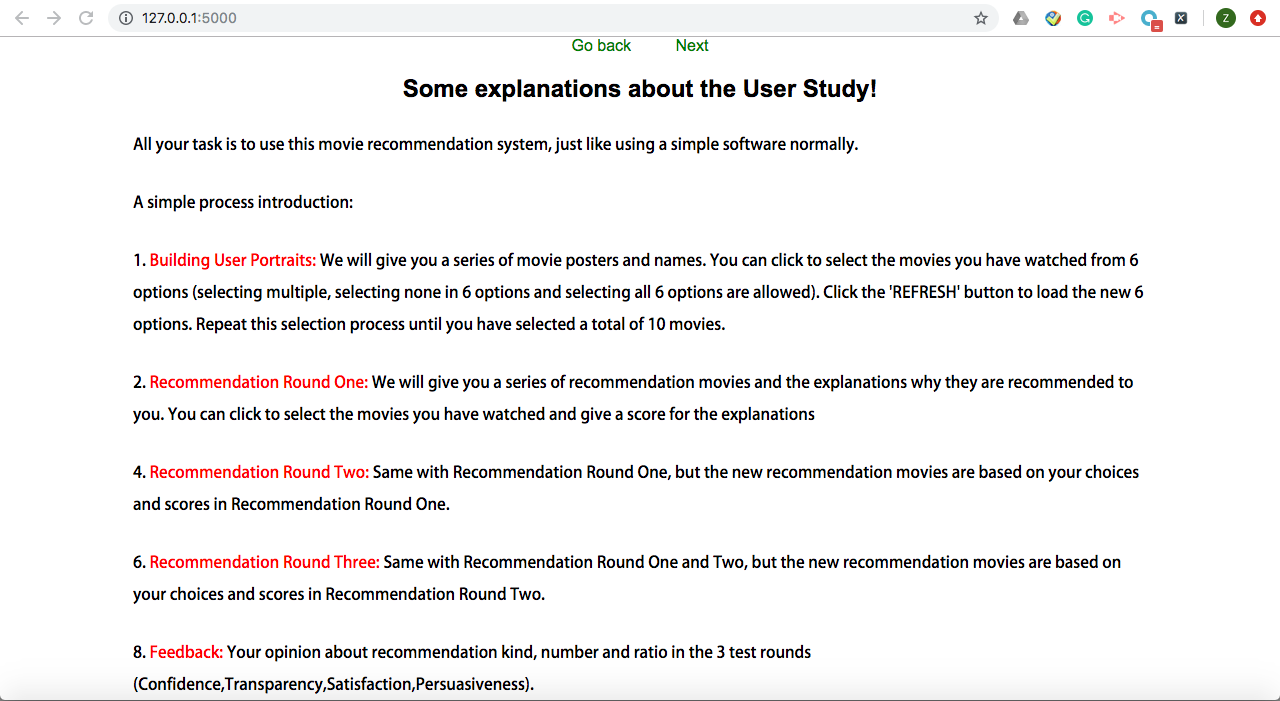
\includegraphics[width=0.8\textwidth]{prototype1}
\end{figure}

\begin{figure}[h]
\caption{User Information Page}
\label{figure:8-2}
\centering
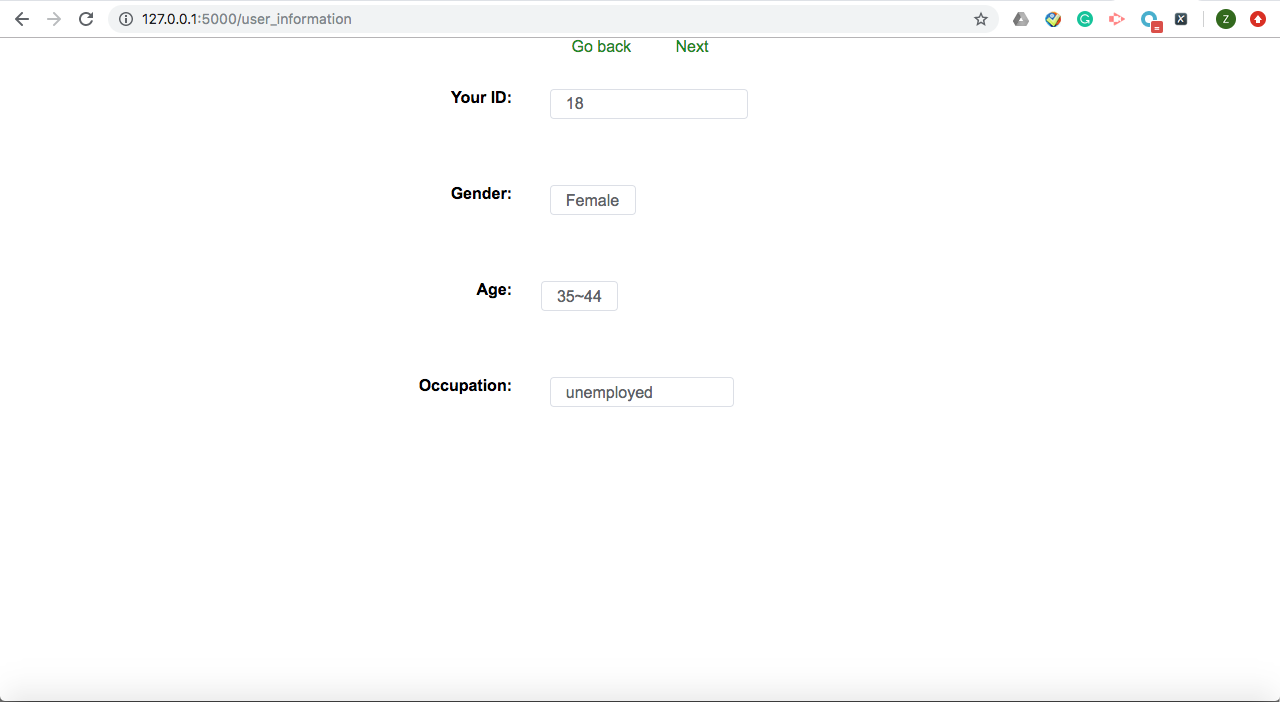
\includegraphics[width=0.8\textwidth]{prototype2}
\end{figure}

\begin{figure}[h]
\caption{User Background Page}
\label{figure:8-3}
\centering
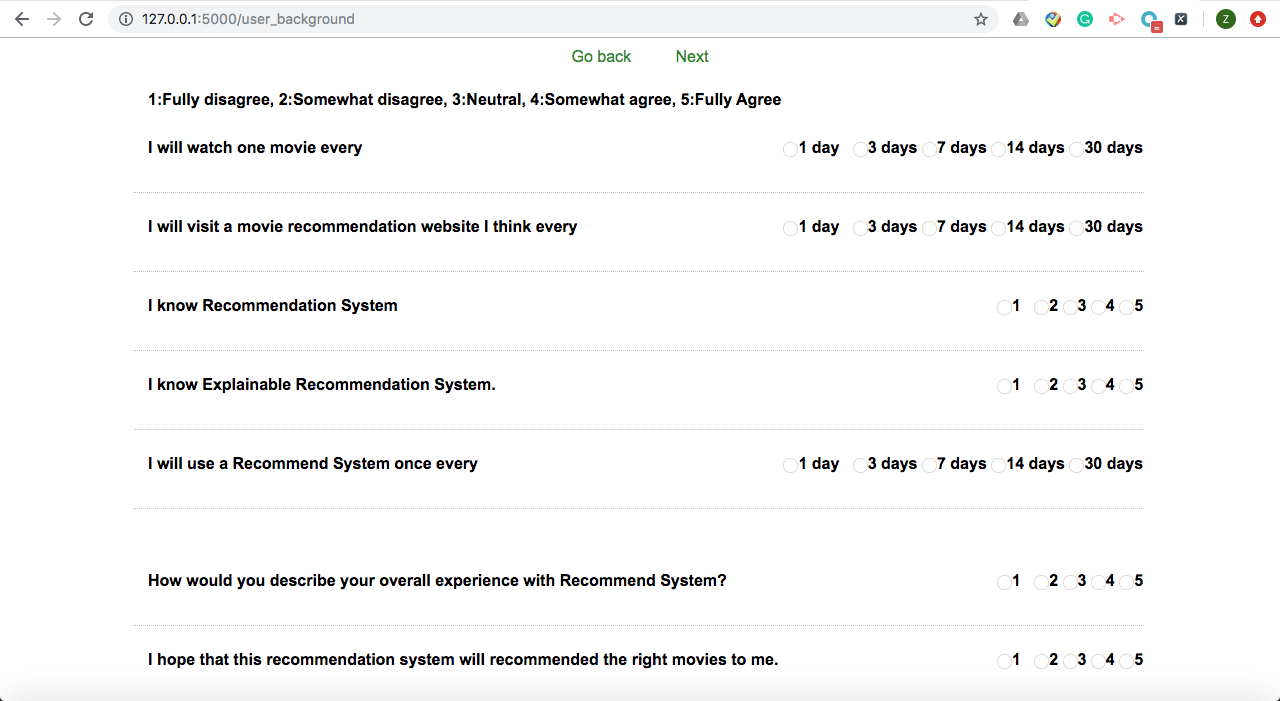
\includegraphics[width=0.8\textwidth]{prototype3}
\end{figure}

\begin{figure}[h]
\caption{Movie Preview Page}
\label{figure:8-4}
\centering
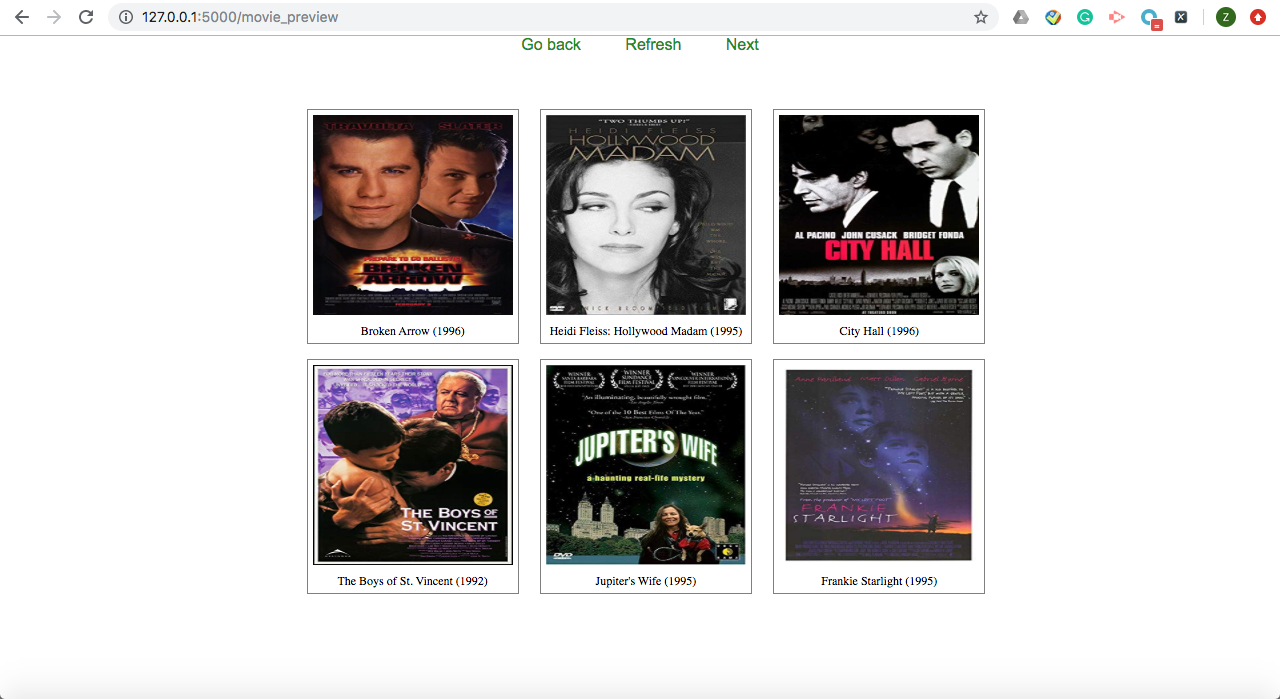
\includegraphics[width=0.8\textwidth]{prototype4}
\end{figure}

\begin{figure}[h]
\caption{Movie Degree Page}
\label{figure:8-5}
\centering
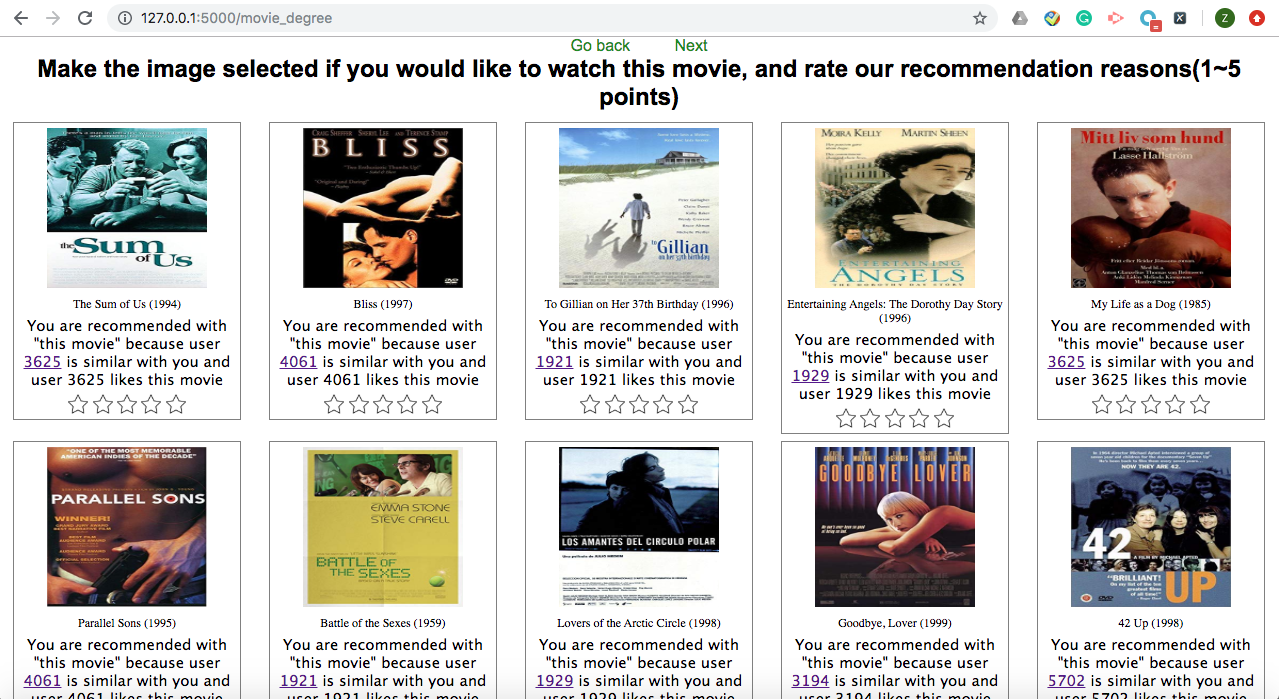
\includegraphics[width=0.8\textwidth]{prototype5}
\end{figure}

\begin{figure}[h]
\caption{Movie Degree Page with scores}
\label{figure:8-6}
\centering
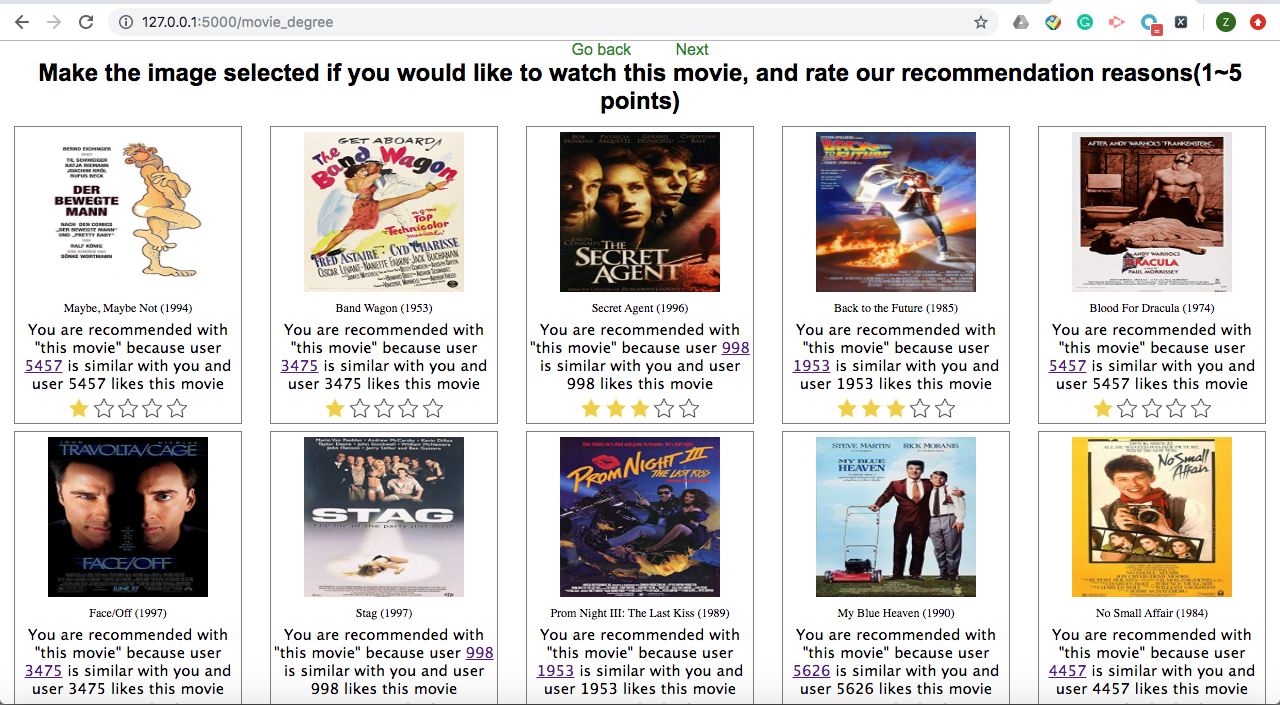
\includegraphics[width=0.8\textwidth]{prototype6}
\end{figure}

\begin{figure}[h]
\caption{Coresponding User Inforamtion Page}
\label{figure:8-7}
\centering
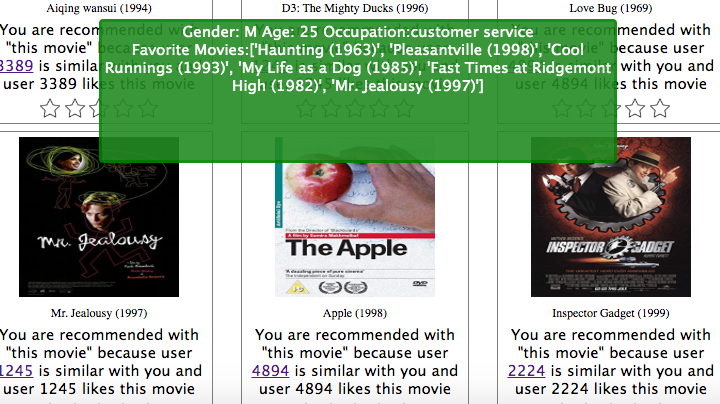
\includegraphics[width=0.8\textwidth]{prototype7}
\end{figure}

\begin{figure}[h]
\caption{User Feedback Page}
\label{figure:8-8}
\centering
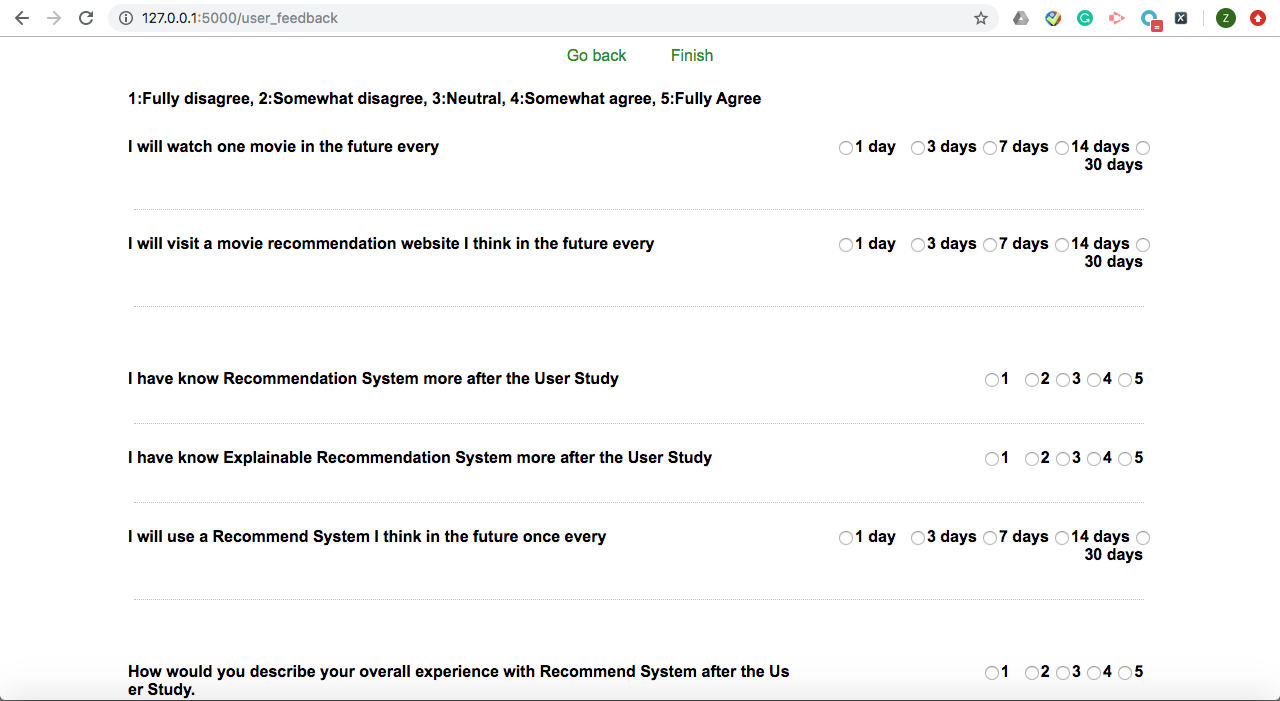
\includegraphics[width=0.8\textwidth]{prototype8}
\end{figure}

\subsection{Raw Data Illustration}

\cleardoublepage